%%%%%%%%%%%%%%%%%%%%%%%%%%%%%%%%%%%%%%%%%
% a0poster Landscape Poster
% LaTeX Template
% Version 1.0 (22/06/13)
%
% The a0poster class was created by:
% Gerlinde Kettl and Matthias Weiser (tex@kettl.de)
% 
% This template has been downloaded from:
% http://www.LaTeXTemplates.com
%
% License:
% CC BY-NC-SA 3.0 (http://creativecommons.org/licenses/by-nc-sa/3.0/)
%
%%%%%%%%%%%%%%%%%%%%%%%%%%%%%%%%%%%%%%%%%

%----------------------------------------------------------------------------------------
%	PACKAGES AND OTHER DOCUMENT CONFIGURATIONS
%----------------------------------------------------------------------------------------

\documentclass[a0,landscape,24pt]{a0poster}

\usepackage{multicol} % This is so we can have multiple columns of text side-by-side
\columnsep=100pt % This is the amount of white space between the columns in the poster
\columnseprule=3pt % This is the thickness of the black line between the columns in the poster

\usepackage[svgnames]{xcolor} % Specify colors by their 'svgnames', for a full list of all colors available see here: http://www.latextemplates.com/svgnames-colors

\usepackage{times} % Use the times font
%\usepackage{palatino} % Uncomment to use the Palatino font

\usepackage{graphicx} % Required for including images
\graphicspath{{figures/}} % Location of the graphics files
\usepackage{booktabs} % Top and bottom rules for table
\usepackage[font=small,labelfont=bf]{caption} % Required for specifying captions to tables and figures
\usepackage{amsfonts, amsmath, amsthm, amssymb} % For math fonts, symbols and environments
\usepackage{wrapfig} % Allows wrapping text around tables and figures

\begin{document}

%----------------------------------------------------------------------------------------
%	POSTER HEADER 
%----------------------------------------------------------------------------------------

% The header is divided into three boxes:
% The first is 55% wide and houses the title, subtitle, names and university/organization
% The second is 25% wide and houses contact information
% The third is 19% wide and houses a logo for your university/organization or a photo of you
% The widths of these boxes can be easily edited to accommodate your content as you see fit

\begin{minipage}[b]{0.75\linewidth}
\veryHuge \color{NavyBlue} \textbf{Continuous Optimization Model for Instruction Scheduling} \color{Black}\\ % Title
\Huge\textit{And Rapid Prototyping in Coconut}\\[2cm] % Subtitle
\huge \textbf{Curtis D'Alves}\\[0.5cm] % Author(s)
\huge \textbf{Dr. Christopher Anand, Dr. Wolfram Kahl}\\[0.5cm] % Author(s)
\huge McMaster University Department of Computing \& Software \\[0.4cm] % University/organization
\Large \texttt{dalvescb@mcmaster.ca} \\
\Large \texttt{anandc@mcmaster.ca, kahl@cas.mcmaster.ca} \\

\end{minipage}
%
\begin{minipage}[b]{0.25\linewidth}

\includegraphics[width=10cm]{maclogo.jpg}\\

\includegraphics[width=20cm]{logo.png}\\
\end{minipage}

\vspace{1cm} % A bit of extra whitespace between the header and poster content

%----------------------------------------------------------------------------------------

\begin{multicols}{3} % This is how many columns your poster will be broken into, a poster with many figures may benefit from less columns whereas a text-heavy poster benefits from more

%----------------------------------------------------------------------------------------
%	ABSTRACT
%----------------------------------------------------------------------------------------

\color{Navy} % Navy color for the abstract

\begin{abstract}

Instruction scheduling is an NP-complete problem which allows for altering the execution order of instructions in a function without altering the function's semantics. By modifying instruction execution order, CPU resource usage can be maximized resulting in increased instruction throughput and decreased overall execution times. We present a continuous optimization based model for solving near-optimal schedules and a prototype implemented for the IBM z13 and z14 architectures. By adopting a continuous optimization model, we can encode many complex / overlapping scheduling heuristics as penalty functions and adjust priority through scaling of those functions while still allowing for a certain flexibility of influence between each heuristic.


\end{abstract}

%----------------------------------------------------------------------------------------
%	Model
%----------------------------------------------------------------------------------------

\color{SaddleBrown} % SaddleBrown color for the introduction

\section*{Overview: Instruction Scheduling}

\begin{center}\vspace{1cm}
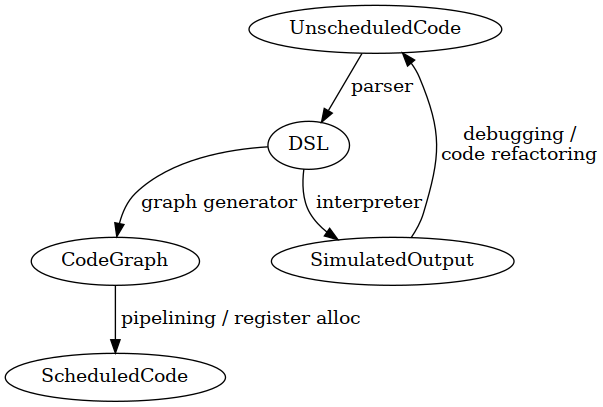
\includegraphics[width=1.0\linewidth,height=0.8\linewidth]{graph}
\captionof{figure}{\color{Green} MASS VCOS Dependency Graph}
\end{center}\vspace{1cm}

\begin{itemize}
	\item It is of interest to distinguish between classes of instructions, including: {\color{red} General Purpose Register Ops}, {\color{Green} Vector Loads/Stores}, {\color{orange} Vector Ops}, {\color{blue} Floating Point Ops}
	\item Given a DAG (Directed Acyclic Graph) representing dependencies between instructions, we seek a {\it schedule} (execution order) satisfying these dependencies while yielding near-optimal performance
	\item The code is an unrolled loop, it is broken up into {\it stages} that are {\it pipelined} together
	\item Many aspects affect performance that need to be considered, including: Register Allocation, Dispatches per cycle of instruction class, Load Latency 
\end{itemize}

%------------------------------------------------
\color{DarkSlateGray} % DarkSlateGray color for the rest of the content

\section*{Model}

    Per Instruction $i$, perform a relaxation of scheduled position to dispatch and completion times $t_i$,$b_i$
    \begin{align*}
    \text{\color{Navy} Objective Variables \qquad} & t_i, b_i, f_i:& \mathbb{R} \\
    \text{\color{Navy} Constants \qquad} & \textrm{II} :& \mathbb{R} \\
    \text{\color{Navy} Indicator Function \qquad} & \mathbb{IN} :& \mathbb{R} \rightarrow \mathbb{R} \\
    & t_i :& \text{dispatch time} \\
    & b_i :& \text{completion time} \\
    & f_i :& \text{FIFO use } 0 \leq f_i \leq 1 \\
    & \textrm{II} :& \text{iteration interval} \frac{\# instructions}{dispatches/cycle} \\
    \end{align*}
    
    \begin{align}
    \text{\color{Navy} Hard Constraints \qquad}  & t_i + \epsilon \leq t_j \qquad & \forall i,j \cdot i \rightarrow j \\
								 & 0 \leq t_i \leq b_i \leq \#\text{stages} \cdot \textrm{II}  & \\
								 & b_i + \epsilon \leq t_i + \textrm{II} \\
    \text{\color{Navy} Objective Function \qquad}   & \text{min} \sum_{i} (t_i + f_i) + \text{Penalties}
    \end{align}




\subsubsection*{Indicator Function}

\begin{equation}
\mathbb{IN}(s,\delta t) = \frac{1}{(1 + e^{s \; (-0.5 + \delta t)}) \cdot (1 + e^{s \; (-0.5 - \delta t)})}
\end{equation}

\begin{center}\vspace{1cm}
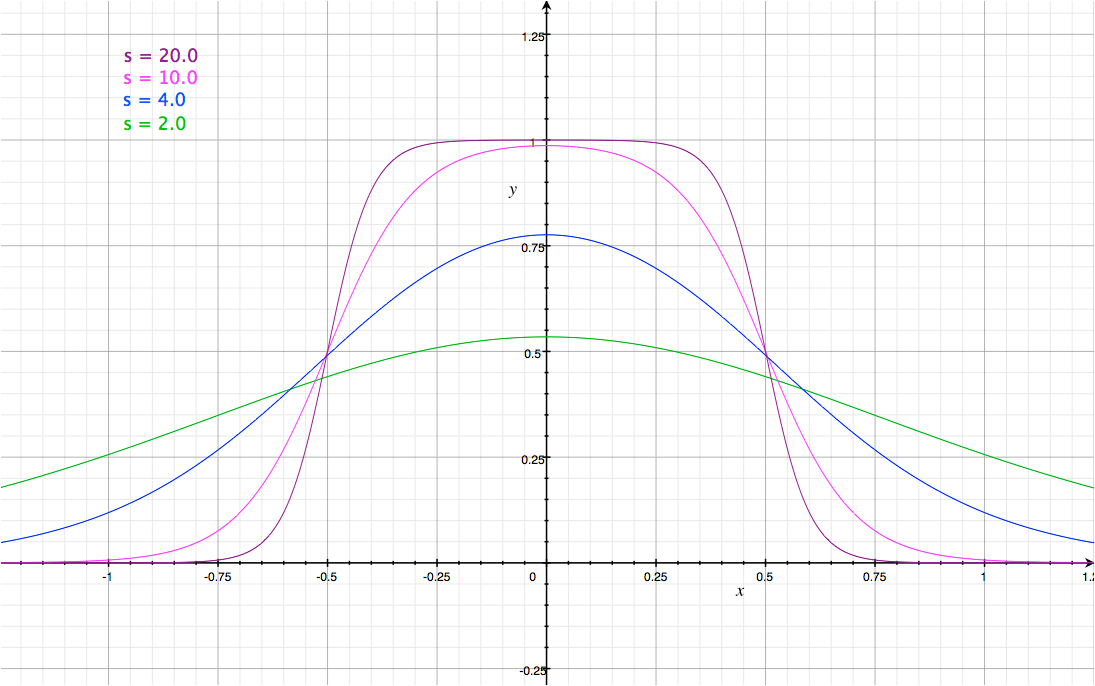
\includegraphics[width=0.7\linewidth]{sigmoid}
\captionof{figure}{\color{Green} Indicator Function $\mathbb{IN}$}
\end{center}\vspace{1cm}

\begin{equation}
\text{\color{Navy} Example: Floating Point Dispatch Penalty} \quad \sum_{i,j \in \text{FP}} \mathbb{IN}(s,t_i - t_j - \textrm{II})
\end{equation}

%----------------------------------------------------------------------------------------
%	RESULTS 
%----------------------------------------------------------------------------------------
\color{Navy}
\section*{Rapid Prototyping With Coconut}

Coconut (COde CONstructing User Tool), is an extensible domain-specific language (DSL) embedded in Haskell we've developed for prototyping scheduling algorithms

\begin{center}\vspace{1cm}
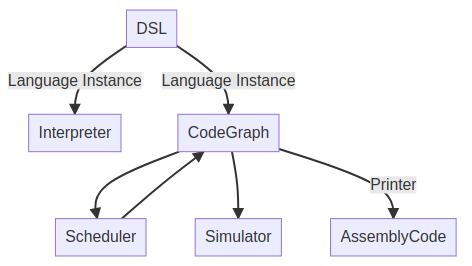
\includegraphics[width=0.7\linewidth]{coconut}
\captionof{figure}{\color{Green} Coconut Prototyping Process}
\end{center}\vspace{1cm}

The DSL provides an interface for experts in high performance numerical software to provide processor-specific implementations of mathematical functions, with the following goals

\begin{itemize}
 \item The language supports type safety, and is familiar to mathematicians
 \item The user is insulated from details of the target intermediate language not relevant to their task
 \item Alternatives for instruction selection can be provided by the user
\end{itemize}	

%----------------------------------------------------------------------------------------
%	FORTHCOMING RESEARCH
%----------------------------------------------------------------------------------------

\color{SaddleBrown} % SaddleBrown color for the conclusions to make them stand out

\section*{Forthcoming Research}

\begin{itemize}
\item Penalties to decide probability of FIFO use to avoid register spilling have not yet been implemented. Viability of a {\it Mixed-Integer Linear Programming}  model could be explored
\item Systematic approaches to selecting scaling of penalties
\item Custom solver for updating smoothing of indicator functions during optimization iterations
\end{itemize}

\color{DarkSlateGray} % Set the color back to DarkSlateGray for the rest of the content


 %----------------------------------------------------------------------------------------
%	REFERENCES
%----------------------------------------------------------------------------------------

\nocite{*} % Print all references regardless of whether they were cited in the poster or not
\bibliographystyle{plain} % Plain referencing style
\bibliography{sample} % Use the example bibliography file sample.bib

%----------------------------------------------------------------------------------------
%	ACKNOWLEDGEMENTS
%----------------------------------------------------------------------------------------

\section*{Acknowledgements}

Special Thanks to IBM's Robert Enenkel and Bill O'Farrell for their assistance. This project seeks to succeed the work of Kriston Costa's Stochastic Approach to Instruction Scheduling. Although the approach was inherently distinct from our own, much was learnt and applied from his attempts.

%----------------------------------------------------------------------------------------

\end{multicols}
\end{document}